\documentclass[12pt,a4paper]{article}

% --- Page Layout ---
\usepackage[margin=1in]{geometry}
\usepackage{setspace}
% \doublespacing

% --- Paragraph Formatting ---
\usepackage{parskip}  % no paragraph indentation, adds vertical space
\setlength{\parindent}{15pt}  % resets indentation 
\usepackage{indentfirst}  % indent first paragraph of sections (optional)

% --- Font and Typography ---
\usepackage{newpxtext,newpxmath}
% \usepackage{times}
\usepackage[T1]{fontenc}
\usepackage[utf8]{inputenc}

% --- Section Title Formatting ---
\usepackage{titlesec}
\titleformat{\section}{\normalfont\Large\bfseries}{\thesection.}{1em}{}
\titleformat{\subsection}{\normalfont\large\bfseries}{\thesubsection.}{1em}{}

% --- Math ---
\usepackage{amsmath, amssymb, amsthm}

% --- Figures and Tables ---
\usepackage{graphicx}
\usepackage{caption}
\usepackage{subcaption}
\usepackage{float}
\usepackage{booktabs}
\usepackage{arydshln}

% --- References ---
% \usepackage{natbib}
% \usepackage[
%     backend=biber,
%     style=authoryear,
%     natbib=true
% ]{biblatex}
% \addbibresource{bibliography.bib}
\usepackage{natbib}
\bibliographystyle{apalike}

% --- Hyperlinks ---
\usepackage{hyperref}
\hypersetup{
    colorlinks=true,
    linkcolor=blue,
    citecolor=blue,
    urlcolor=blue
}

% --- Theorems ---
\newtheorem{theorem}{Theorem}
\newtheorem{proposition}{Proposition}
\newtheorem{lemma}{Lemma}

 % --- Header/Footer (optional for working papers) ---
% \usepackage{fancyhdr}
% \pagestyle{fancy}
% \fancyhead[L]{Working Paper}
% \fancyhead[R]{\thepage}

% --- Rotating tables ---
\usepackage{rotating} % Needed for sidewaystable

\title{Is Peru's FX Intervention Optimal? A Calibrated Framework}
\author{Gonzalo Bueno Bustíos}
\date{March 2025}

\begin{document}

\maketitle

\section{Introduction}

In recent years, due to significant movements of capital around the world, Central Banks have been keen on participating in the FX market. This has evoked questions regarding what the optimal FX policy to implement is. Does this policy maximize welfare? What are the optimal policy tools to implement it? Through what channels do these tools operate?

This essay analyzes the case of the Peruvian Central Bank. The institution has is particularly active with FX interventions to reduce exchange rate volatility, through selling or buying USD or using swaps that keep international reserves untouched. This has been a success case. Compared to the rest of South America, Peru has had one of the lowest depreciations as well as less volatility in recent years.

\begin{figure}[H]
    \centering
    \caption{FX Trends over time}
    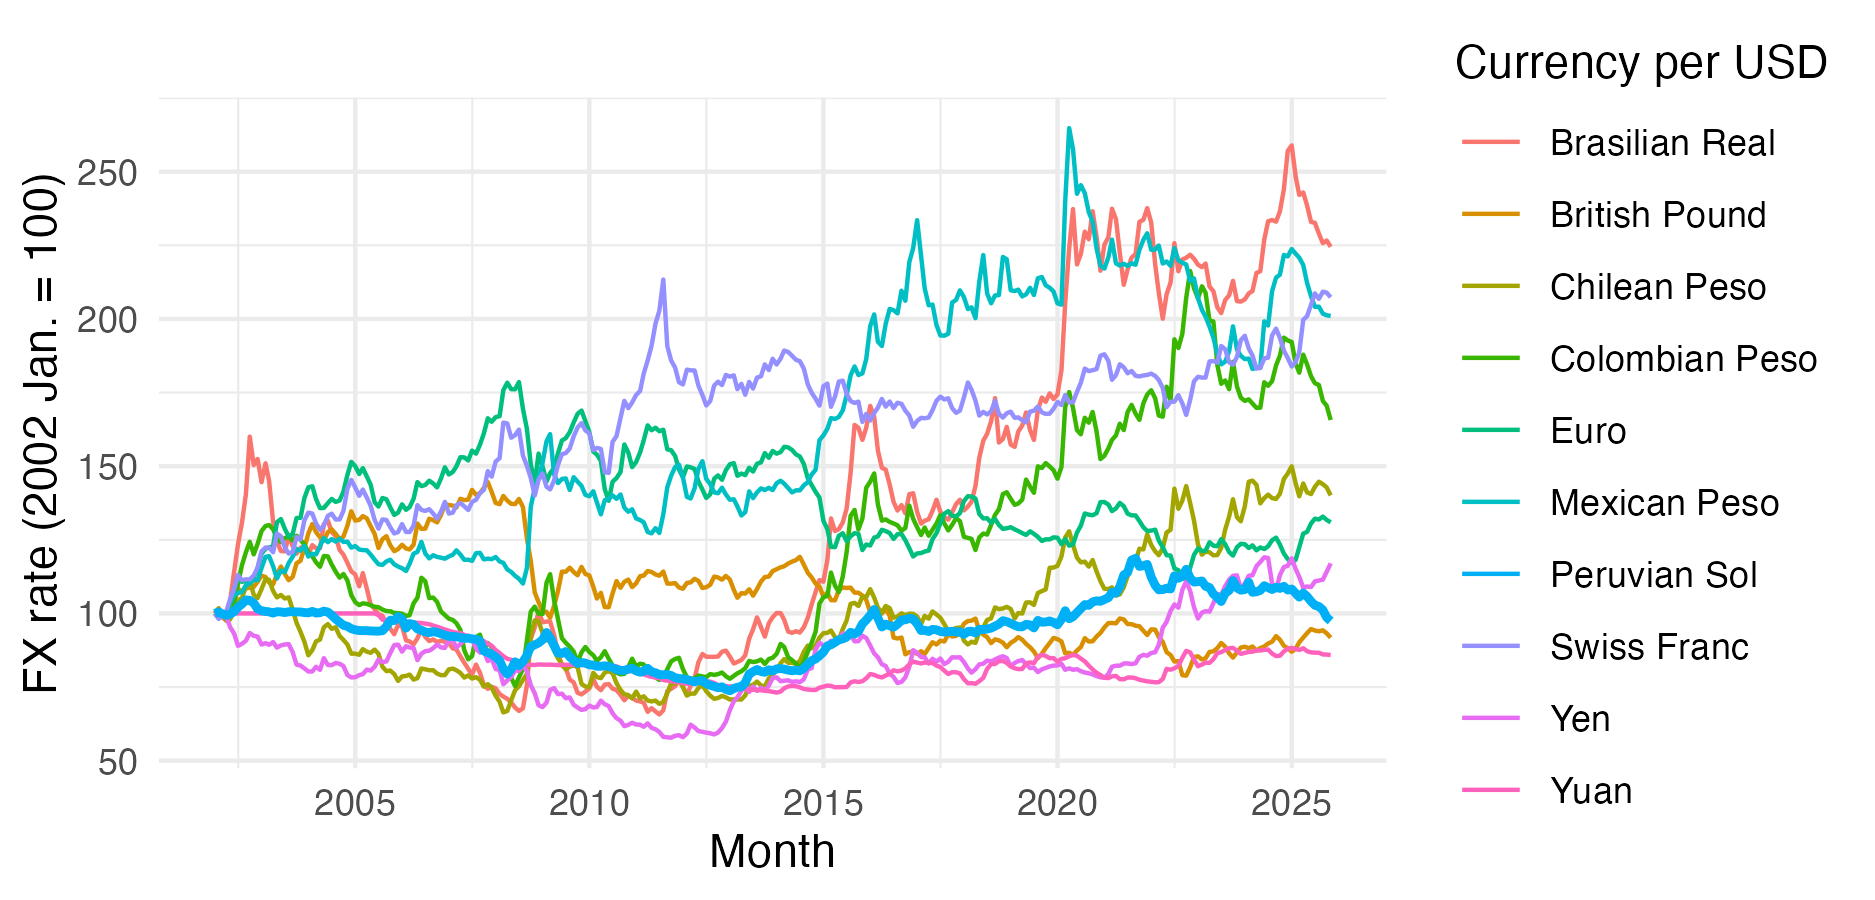
\includegraphics[width=\linewidth]{figures/fx_plot.png}     \label{fig:fx_plot}
    \smallskip
    \begin{minipage}{0.95\linewidth}
    \footnotesize
    \textit{Notes:} This figure depicts the exchange rate per USD for ten economies from 2002 to 2025 normalized to January 2002 $= 100$. The thicker line corresponds to the Peruvian Sol, which has had the most stable value over the period. The sample includes the following countries: Peru, Brazil, Chile, Colombia, Mexico, Euro Area, Japan, UK, Switzerland, and China.
  \end{minipage}
 \end{figure}


From 2002 to 2025 (implementation of Inflation Targeting in Peru), the volatility of the USD/Peruvian Sol exchange rate has been 1.3\footnote{This has been measured as the standard deviation of the log variation of the interest rate normalized to 100.}, which is 1.7 and 2.41 times the average volatility of developed countries (excluding China) and emerging economies respectively.

\begin{table}[htbp]
  \centering
  \caption{Exchange Rate to USD Volatility}
  \label{tab:fx_volatility}
  \begin{tabular}{lc}
    \toprule
    Currency & Volatility (\%) \\
    \midrule
    Peruvian Sol  & 1.30 \\
    \midrule
    \multicolumn{2}{l}{\textit{Developed economies}} \\
    Euro          & 2.14 \\
    Japanese Yen  & 2.15 \\
    British Pound & 3.78 \\
    Swiss Franc   & 2.76 \\
    Chinese Yuan  & 2.20 \\
    \midrule
    \multicolumn{2}{l}{\textit{Emerging economies}} \\
    Brazilian Real  & 2.29 \\
    Chilean Peso    & 2.74 \\
    Colombian Peso  & 0.85 \\
    Mexican Peso    & 3.23 \\
    \midrule
    \bottomrule
  \end{tabular}
  \smallskip
  \begin{minipage}{\linewidth}
    \small
    \textit{Notes:} Volatility is computed as the standard deviation of log
    first-differences of monthly bilateral exchange rates against the US dollar,
    multiplied by 100. Sample period: 2002--2025.
  \end{minipage}
\end{table}

This has been a particular challenge, as the Peruvian economy is a partially dollarized one (by September of 2025, 25.5 percent of credit issued to the private sector is in USD). This means that there exists a balance sheet effect of exchange rate volatility over firms, which creates an incentive for the Central Bank to intervene in FX markets to reduce volatility and therefore eliminate a potential channel from where risk can impact the real economy or create a stronger feedback effect over USD depreciation.

\begin{figure}[H]
    \centering
    \caption{Dollarization rate}
    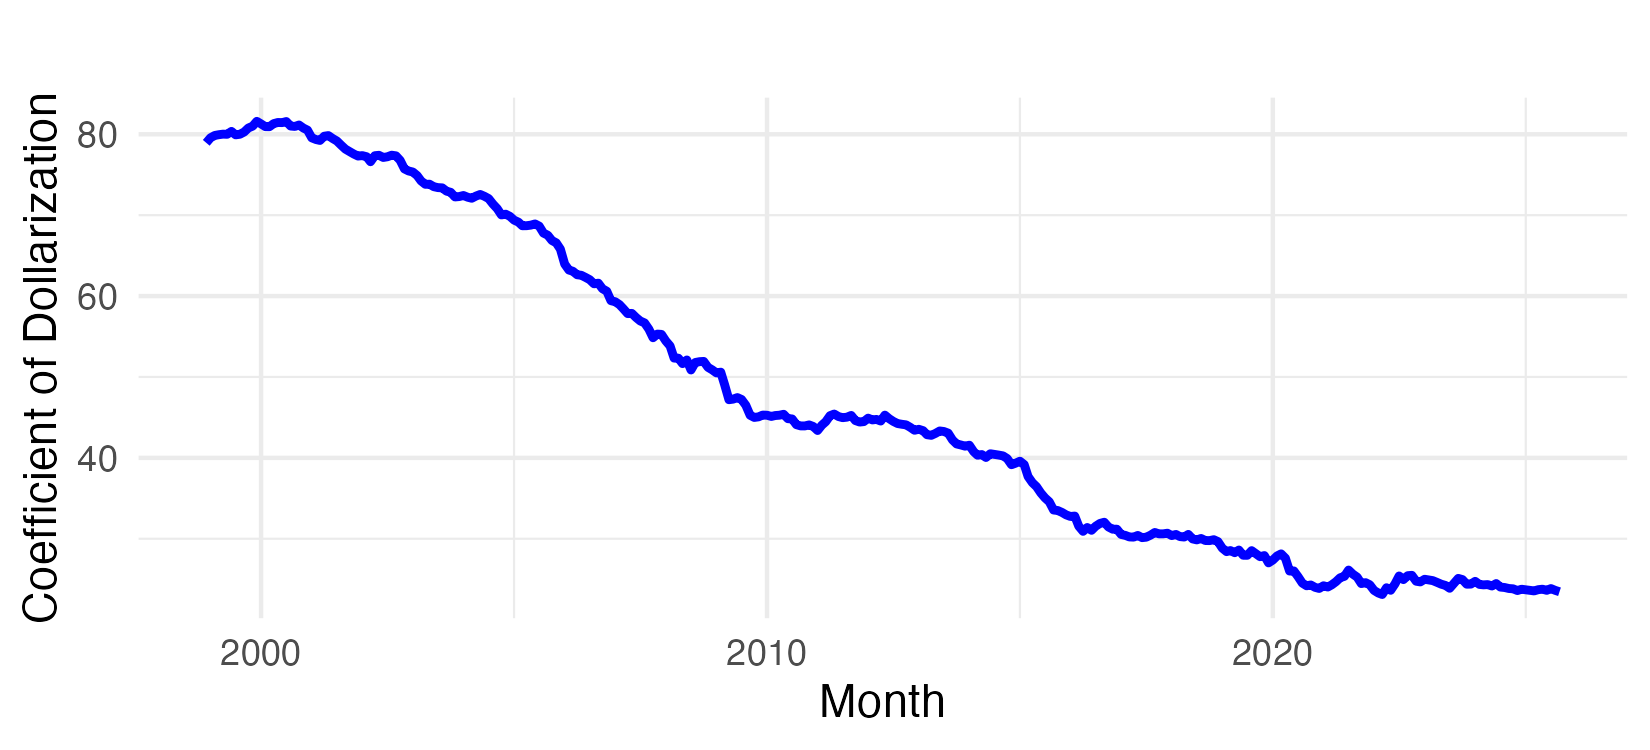
\includegraphics[width=0.85\linewidth]{figures/doll_plot.png }     \label{fig:doll_plot}
 \end{figure}

This case has already been subject to study. In \cite{MONTORO2023102825}, a New Keynesian small open economy model with financial intermediaries as in \cite{doi:10.1086/714447} is used to generate deviations from UIP. The authors show that shocks can trigger inefficient FX paths and that policy responses can increase welfare.

\subsection{Theoretical framework and research question}

The research question of this essay will be: has the FX policy of the Peruvian Central Bank been optimal? 

This project will be done in four stages:

\begin{enumerate}
    \item \textbf{Deeper review of existing literature.} The current literature review has been based on recent results of the current state of the academic debate. In the first stage, I will enrich the literature with theoretical papers that support the modeling decisions and similar case studies.
    
    \item \textbf{Theoretical model.} In the essay, I will elaborate on a simplified version of \cite{itskhokimukhin2025} that captures the policy decision of a Central Bank. It will minimize a loss function between the output gap (or a measure that relies on sticky prices, such as actual inflation relative to the target) and a wedge that measures deviations from UIP. The restrictions will come from: (1) risk-sharing conditions [international access to foreign markets], (2) allocation of consumption between tradables and non-tradables [equilibrium in the goods market], and (3) equilibrium in the financial market. It is in this case where intervention in the FX market can absorb the shocks that create deviations from UIP due to capital flows in the financial market. I will prioritize having an analytically simple form of the model that will allow for a detailed analysis of how it works. The equations will be derived, but the main theorems explored in \cite{itskhokimukhin2025} will be used as given.
    
    \item \textbf{Stylized facts and calibration.} Using literature on estimation and calibration of Peruvian models (in particular \cite{MONTORO2023102825} already has some results that can be useful), some parameters will be recovered. The remaning parameters of the model will be either estimated through simple OLS regressions or calibrated such that they match how data behaves. Due to the limitations on time and scope of this essay the calibration will not be extensive. An opportunity to expand and improve the essay would be the use of stronger methods, like Bayesian econometrics, to estimate the parameters of the model.
    
    \item \textbf{Comparison of policy reactions to shocks and measurements of welfare.} Four episodes will be contrasted: the 2008 financial crisis, the taper tantrum, the 2020 pandemic, 2021 elections. I will simulate shocks of the same magnitude and estimate what the model predicts is the correct strategy and contrast it with the actual policy path. Then, a measure of welfare can be recovered from the loss function of the Central Bank.
    
\end{enumerate}

This essay aims to shed light on the literature through the calibration of a novel model to estimate the optimal FX policy for a particular country. Differently from \cite{MONTORO2023102825}, where they discard optimal rules from a central bank optimization problem, I will contrast the results with the policy resulting from \cite{itskhokimukhin2025}.

\section{Theoretical framework}

This section introduces the model that will be used in the essay. It follows the \cite{itskhokimukhin2025} model that captures the policy decision of a Central Bank over the use of monetary policy and FX interventions.

\subsection{The economy}

The model describes a small open economy with four types of agents: households, arbitrageurs (financial intermediaries), noise traders, and a government that includes the central bank. The key structural feature is segmentation in global asset markets: domestic households have access only to local-currency bonds, so all international capital flows must be intermediated by the arbitrageurs. This segmentation is what generates endogenous deviations from uncovered interest rate parity (UIP) and creates a role for FX intervention.

\paragraph{Households.} A representative household derives utility from consumption of non-tradable goods $C_{Nt}$ and tradable goods $C_{Tt}$
\begin{equation}
    U_t = \gamma \log C_{Tt} + (1-\gamma) \log C_{Nt},
    \label{eq:utility}
\end{equation}
where $\gamma \in (0,1)$ measures the openness of the economy, i.e.\ the weight placed on tradable consumption. The household supplies labor inelastically to non-tradable production and receives profits from firms. Crucially, the household can only save and borrow using the home-currency bond $B_t$ at the domestic nominal interest rate $R_t$; it has no direct access to foreign-currency assets.

\paragraph{Goods market.} Non-tradable output $Y_{Nt} = C_{Nt}$ clears domestically. Under fully sticky non-tradable prices ($P_{Nt} = 1$) and the law of one price for tradables ($P_{Tt} = E_t P^*_{Tt}$), the optimal expenditure allocation between tradables and non-tradables implies:
\begin{equation}
    E_t = \frac{\gamma}{1-\gamma} \cdot \frac{C_{Nt}}{C_{Tt}},
    \label{eq:expenditure}
\end{equation}
so that the nominal exchange rate $E_t$ is the relative price that clears the goods market. %Equation~\eqref{eq:expenditure} is log-linear in the endogenous variables: any gap in either $C_{Nt}$ or $C_{Tt}$ relative to their first-best levels translates directly into exchange rate misalignment.

\paragraph{Financial intermediaries (arbitrageurs).} Arbitrageurs can hold both home and foreign currency bonds, but face a mean-variance portfolio problem with risk-aversion parameter $\omega > 0$. Their optimal carry-trade position $D^*_t/R^*_t$ satisfies
\begin{equation}
    \frac{D^*_t}{R^*_t} = \frac{\mathbb{E}_t[\Theta_{t+1}\tilde{R}^*_{t+1}]}{\omega \sigma^2_t},
    \label{eq:arbitrageur}
\end{equation}
where $\Theta_{t+1} = \beta C_{Tt}/C_{Tt+1}$ is the stochastic discount factor of households, $\tilde{R}^*_{t+1} = R^*_t - R_t E_t/E_{t+1}$ is the return on one dollar of carry trade, and $\sigma^2_t \equiv \text{var}_t(\Delta e_{t+1})$ is the conditional exchange rate variance. %As $\omega \to 0$ the market becomes frictionless and UIP holds exactly. For $\omega > 0$, arbitrageurs demand a risk premium in proportion to both their net exposure and the level of exchange rate volatility, which is the core friction of the model.

\paragraph{Noise traders and the government.} Noise traders generate exogenous currency demand shocks $N^*_t$ that represent non-fundamental capital flows. The government (central bank) holds net foreign currency assets $F^*_t$ via sterilised FX interventions. Financial market clearing requires:
\begin{equation}
    D^*_t + F^*_t + N^*_t = B^*_t,
    \label{eq:fmclearing}
\end{equation}
where $B^*_t$ is the net foreign asset (NFA) position of domestic households intermediated through the financial sector. Sterilisation means that FX purchases or sales by the central bank do not affect the domestic monetary base.%, so they work purely through the portfolio-balance channel: by absorbing or injecting foreign currency supply, the government shifts the net exposure borne by arbitrageurs and thus changes the risk premium they demand.

\paragraph{First-best allocation and the risk-sharing wedge.} The first-best allocation $\{\tilde{C}_{Nt}, \tilde{C}_{Tt}, \tilde{B}^*_t\}$ is defined as the equilibrium that obtains when $\omega = 0$, so that UIP holds and households can smooth tradable consumption at the world interest rate $R^*_t$. Deviations from this benchmark are captured by two wedges: the \textit{output gap} $x_t \equiv \log(C_{Nt}/\tilde{C}_{Nt})$, which measures the cost of nominal rigidities in the goods market, and the \textit{risk-sharing wedge} $z_t \equiv \log(C_{Tt}/\tilde{C}_{Tt})$, which measures the distortion to tradable consumption caused by financial frictions. When $z_t < 0$, households consume fewer tradables than is socially optimal because arbitrageurs charge a premium for intermediating capital flows; when $z_t > 0$ the opposite holds.

The frictional UIP condition (obtained by combining household and arbitrageur optimality with financial market clearing) shows that the expected change in the risk-sharing wedge equals the UIP deviation:
\begin{equation}
    i_t - i^*_t - \mathbb{E}_t \Delta e_{t+1} = \mathbb{E}_t \Delta z_{t+1},
    \label{eq:uip_wedge}
\end{equation}
so the risk-sharing wedge and the UIP premium are two sides of the same friction: the risk premium charged by arbitrageurs is precisely what prevents households from achieving efficient risk sharing.

\subsection{The policy problem}

The Central Bank has two tools to intervene in the economy: (1) a standard interest rate policy, and (2) an FX intervention that can absorb shocks that create deviations from UIP due to capital flows in the financial market. The Central Bank minimizes a loss function between the output gap (or a measure that relies on sticky prices, such as actual inflation relative to the target) and a wedge that measures deviations from UIP.

\cite{itskhokimukhin2025} presents the policy problem as deviations from a first-best allocation. The Central Bank's problem is to choose a policy that minimizes the loss function subject to the constraints of the economy.

The loss function is given by:

\begin{equation}
    L = \frac{1}{2}\mathbb{E}\sum_{t=0}^{\infty} \beta^t \left[ \gamma z_t^2 + (1-\gamma) x_t^2 \right]
\end{equation}

where $z_t$ is the risk sharing wedge and $x_t$ is the output gap, $\beta$ is the discount factor, and $\gamma$ is a parameter that captures the relative weight of the two components of the loss function.

This function is minized with the following constraints from the economy solution:

\begin{itemize}
    \item Country budget constraint (exports-imports as counterpart of the net foreign asset position): 
    $\beta b_t^* = b_{t-1}^* - z_t$.
    
    \item Expenditure allocation condition in the goods market: 
    $e_t = \bar{q_t} + x_t - z_t$.
    
    \item Equilibrium in the financial market:
    $\mathbb{E}_t \Delta (z_{t+1}) = \bar{\omega} \bar{\sigma_t^2} (n_t^* + f_t^* - b_t^*)$.

\end{itemize}

The first-best allocation is achieved when $z_t = 0$ and $x_t = 0$ for all $t$. Any additional constraints on the FX intervention will create deviation from the best-case scenario. 

The Ramsey optimal monetary policy for any given FX intervention rule satisfies the following conditions:

\begin{itemize}
    \item Output gap: $x_{t+1} = -\delta_t (e_{t+1} - \mathbb{E}_t e_{t+1})$.
    \item Intensity of monetary policy lean: $\delta_t = \frac{2 \gamma \bar{\omega}}{1 - \gamma} \frac{\bar{\omega} \bar{\sigma}_t^2}{1 + \beta + \bar{\omega} \bar{\sigma}_t^2} (n_t^* + f_t^* - b_t^*)$.
\end{itemize}
    
This corresponds as the optimal policy response when FX interventions are constrainted. In the case of the Peruvian Central Bank, there is a limit in both the amount of reserves available as well as the amount of information available to compensate noise shocks that lead to increased volatility. This can be interpreted as a FX intervention rule $f_t^* = -\phi n_t^*$. The montery interest rate movements can be recovered from the path of UIP deviations: $i_t - i_t^* - \mathbb{E}_t \Delta e_{t+1} = \mathbb{E}_t \Delta (z_{t+1})$.

\subsection{Model Equations}

The model consists of the following equations:

\begin{enumerate}

    \item \textbf{Exchange rate determination (goods market clearing):}
    \begin{equation}
        e_t = \tilde{q}_t + x_t - z_t
        \label{eq:er}
    \end{equation}

    \item \textbf{NFA dynamics (budget constraint):}
    \begin{equation}
        \beta b^*_t = b^*_{t-1} - z_t
        \label{eq:nfa}
    \end{equation}

    \item \textbf{Risk-sharing condition (financial market clearing):}
    \begin{equation}
        \mathbb{E}_t \Delta z_{t+1} = \bar{\omega}\,\bar{\sigma}^2_t
        \left(n^*_t + f^*_t - b^*_t\right)
        \label{eq:risksharing}
    \end{equation}

    \item \textbf{Endogenous exchange rate volatility:}
    \begin{equation}
        \bar{\sigma}^2_t = \text{Var}_t\left(\Delta e_{t+1}\right)
        \label{eq:sigma}
    \end{equation}

    \item \textbf{Output gap --- monetary policy lean:}
    \begin{equation}
        x_{t+1} = -\delta_t \left(e_{t+1} - \mathbb{E}_t e_{t+1}\right)
        \label{eq:outputgap}
    \end{equation}

    \item \textbf{Intensity of monetary policy lean:}
    \begin{equation}
        \delta_t = \frac{2\gamma\bar{\omega}}{1-\gamma}
        \cdot \frac{\bar{\omega}\bar{\sigma}^2_t}{1 + \beta + \bar{\omega}\bar{\sigma}^2_t}
        \cdot \left(n^*_t + f^*_t - b^*_t\right)
        \label{eq:delta}
    \end{equation}

    \item \textbf{Terms-of-trade shock (AR(1) process):}
    \begin{equation}
        \tilde{q}_t = \rho_q\, \tilde{q}_{t-1} + \varepsilon^q_t
        \label{eq:qtilde}
    \end{equation}

    \item \textbf{Capital flow shock (AR(1) process):}
    \begin{equation}
        n^*_t = \rho_n\, n^*_{t-1} + \varepsilon^n_t
        \label{eq:nstar}
    \end{equation}

    \item \textbf{FX intervention rule (partial offset):}
    \begin{equation}
        f^*_t = -\phi\, n^*_t
        \label{eq:fxi}
    \end{equation}
    where $\phi$ governs the degree to which the central bank
    offsets exogenous currency demand shocks through sterilised FX intervention.

\end{enumerate}

\section{Data and calibration}

\subsection{Data sources}

The empirical analysis draws on quarterly data for Peru covering the period 2002Q1--2024Q4, which spans the full inflation-targeting regime of the Banco Central de Reserva del Per\'u (BCRP). %All series are obtained from the BCRP's public statistical database unless otherwise noted.

The following variables are used. The \textit{nominal exchange rate} is the quarterly average PEN/USD spot rate. \textit{FX intervention volumes} are measured as BCRP net spot purchases of US dollars (in USD millions), with negative values indicating net USD sales; swap operations are recorded separately but included in total intervention. The \textit{terms of trade} index is constructed from export and import price indices published by BCRP and serves as the primary proxy for the fundamental shock $\tilde{q}_t$. \textit{Gross domestic product} is real quarterly GDP (base year 2007). The \textit{trade balance} is measured as a share of GDP. For the external financial environment, the CBOE Volatility Index (VIX) is obtained from the Federal Reserve Economic Data (FRED) and used as a proxy for the capital flow shock $n^*_t$, following the approach of \cite{MONTORO2023102825}.

\subsection{Calibration}

Several parameters of the model are set using a combination of standard values from the literature on small open economies, Peru-specific estimates, and data moments. Table~\ref{tab:calibration} summarises the baseline calibration.

\paragraph{Preference parameters.} The discount factor is set to $\beta = 0.99$, implying an annual real interest rate of approximately 4\%, consistent with Peru's long-run average real interest rate over the sample. The openness parameter $\gamma$ is calibrated to match the share of tradable consumption in total spending; using BCRP national accounts data this yields $\gamma \approx 0.35$, in line with estimates for other commodity-exporting emerging markets.

\paragraph{Financial friction.} The key parameter $\bar{\omega} = \omega_0 \bar{Y}_T / \beta$ governs the price of FX risk. Following \cite{MONTORO2023102825}, who set the absolute risk aversion of FX dealers to 500 in their calibration of a comparable Peru model, we use this as a starting value and refine the estimate empirically using the augmented UIP regression described in Section~\ref{sec:tests}. Because $\bar{\omega}$ determines the strength of the portfolio-balance channel and therefore the welfare gains from FX intervention, obtaining a credible Peru-specific estimate is a central empirical contribution of this essay.

\paragraph{Shock processes.} The persistence and standard deviation of the terms-of-trade shock $(\rho_q, \sigma_q)$ are estimated by fitting an AR(1) to the HP-filtered log terms-of-trade series. This yields $\hat{\rho}_q \approx 0.80$ and $\hat{\sigma}_q \approx 0.03$. %The capital flow shock persistence $\rho_n$ is set to match the autocorrelation of the VIX over the sample, giving $\rho_n \approx 0.90$; the standard deviation $\sigma_n$ is calibrated to match the observed variance of BCRP net intervention volumes under the assumption that $f^*_t \approx -n^*_t$ in the first-best regime, following the insight that backing out $n^*_t$ from observed intervention data provides more realistic Peru-specific estimates than relying solely on VIX moments.

\paragraph{FX intervention intensity.} The partial-offset coefficient $\phi$ in equation~\eqref{eq:fxi} is estimated by projecting BCRP intervention volumes on the identified capital flow shock series. The resulting estimate $\hat{\phi}$ is reported in Table~\ref{tab:calibration} and serves as the empirical counterpart to the optimal $\phi^* = 1$ predicted by the first-best intervention rule.

\begin{table}[H]
    \centering
    \caption{Baseline calibration}
    \label{tab:calibration}
    \begin{tabular}{llll}
        \toprule
        Parameter & Symbol & Value & Source \\
        \midrule
        Discount factor & $\beta$ & 0.99 & Standard \\
        Openness & $\gamma$ & 0.35 & BCRP national accounts \\
        ToT shock persistence & $\rho_q$ & 0.80 & AR(1) on HP-filtered ToT \\
        ToT shock s.d. & $\sigma_q$ & 0.03 & AR(1) on HP-filtered ToT \\
        Capital flow shock persistence & $\rho_n$ & 0.90 & VIX autocorrelation \\
        Capital flow shock s.d. & $\sigma_n$ & 0.01 & BCRP intervention moments \\
        FX risk price & $\bar{\omega}$ & TBE & Augmented UIP regression \\
        Intervention intensity & $\phi$ & TBE & Projection on $n^*_t$ \\
        \bottomrule
        \multicolumn{4}{l}{\footnotesize TBE = to be estimated; see Section~\ref{sec:tests}.}
    \end{tabular}
\end{table}

\section{Model estimation}
\label{sec:estimation}

The linearised equilibrium system -- equations~\eqref{eq:er}--\eqref{eq:fxi} -- is treated as a DSGE model with one non-linear fixed-point equation for $\bar{\sigma}^2_t$ that requires iterative solution. The fixed-point iteration proceeds as follows: given a conjectured value for $\bar{\sigma}^2$, the model is solved, the implied variance of $\Delta e_{t+1}$ is computed analytically from the second moments of the state space solution, and the conjecture is updated until convergence. Convergence is achieved to a tolerance of $10^{-8}$ in all policy regimes considered.

Four policy regimes are simulated and compared:

\begin{enumerate}
    \item \textbf{First-best intervention} ($\phi = 1$): the central bank fully offsets capital flow shocks, $f^*_t = -n^*_t$, and uses monetary policy to close the output gap. This achieves $z_t = x_t = 0$ and represents the welfare benchmark.

    \item \textbf{Free float} ($\phi = 0$, $f^*_t = 0$): no FX intervention; monetary policy follows an inflation-targeting rule. Exchange rate volatility is highest and the risk-sharing wedge is largest.

    \item \textbf{Partial intervention} ($\phi = \hat{\phi}$): the central bank offsets only a fraction $\hat{\phi}$ of capital flow shocks, matching estimated BCRP behaviour. This is the empirically relevant regime and generates a welfare loss intermediate between the first-best and the free float.
\end{enumerate}

Impulse response functions to a one-standard-deviation capital flow shock and to a one-standard-deviation terms-of-trade shock are generated for each regime and reported in Section~\ref{sec:results}.

\section{Empirical Tests}
\label{sec:tests}

This section provides four empirical tests that evaluate whether the theoretical predictions of the model are consistent with observed Peruvian data. The tests are organised from most to least central to the core mechanism of the framework.

\subsection{Test 1: Does BCRP intervention respond to capital flow shocks?}

The first and most direct prediction of the model is that optimal FX intervention offsets non-fundamental capital flow shocks: $f^*_t = -\phi n^*_t$ with $\phi > 0$. To test this, I estimate:
\begin{equation}
    \text{FXI}_t = \alpha + \beta_1 \cdot \text{VIX}_t + \beta_2 \cdot \Delta\text{CapFlow}_t + \varepsilon_t,
    \label{eq:test1}
\end{equation}
where $\text{FXI}_t$ is BCRP net USD purchases (negative = sales), $\text{VIX}_t$ proxies the capital flow shock $n^*_t$, and $\Delta\text{CapFlow}_t$ is the quarterly change in non-resident holdings of Peruvian government bonds (BTP), available from BCRP. The model predicts $\beta_1 < 0$ (the central bank sells USD when global risk rises) and $\beta_2 < 0$ (intervention offsets capital outflows).

\subsection{Test 2: Does FX intervention reduce exchange rate volatility?}

The second prediction is that FX intervention reduces conditional exchange rate variance, $\bar{\sigma}^2_t$. I construct a measure of quarterly conditional exchange rate volatility using a GARCH model estimated on daily PEN/USD data, and then estimate:
\begin{equation}
    \hat{\sigma}^2_t = \alpha + \beta \cdot |\text{FXI}|_t + \gamma \cdot \text{VIX}_t + \varepsilon_t.
    \label{eq:test2}
\end{equation}
The model predicts $\beta < 0$. The reverse-causality problem -- BCRP intervenes more when volatility is already high, which would bias $\beta$ upward -- is addressed by using event studies around major intervention episodes (2008 global financial crisis, 2013 taper tantrum, 2020 COVID shock, 2021 political crisis), exploiting the timing of policy responses relative to external triggers as a quasi-natural experiment.

\subsection{Test 3: UIP deviations and the financial friction mechanism}

The I-M model makes a sharp prediction about when UIP should fail and by how much: deviations from parity are driven by the frictional risk premium $\bar{\omega}\bar{\sigma}^2_t D^*_t$, where $D^*_t \equiv n^*_t + f^*_t - b^*_t$ is the net currency exposure absorbed by arbitrageurs. This prediction has two empirically distinguishable components. First, UIP deviations should be systematically larger during episodes of high exchange rate volatility. Second, and more distinctively, they should be larger precisely when the BCRP is intervening heavily, because heavy intervention signals a large underlying $D^*_t$ that the financial sector must absorb. A model without financial market segmentation (i.e.\ $\bar{\omega} = 0$) predicts neither pattern. This test checks both.

\paragraph{Step 1: Documenting the UIP puzzle for Peru.} I first establish the baseline UIP failure by estimating:
\begin{equation}
    \Delta e_{t+1} = \alpha + \beta_1 (i_t - i^*_t) + \varepsilon_{t+1},
    \label{eq:uip_classic}
\end{equation}
where $\Delta e_{t+1}$ is the log change in the PEN/USD rate, $i_t$ is the BCRP reference rate, and $i^*_t$ is the US federal funds rate. The standard result is $\hat{\beta}_1 < 0$ — currencies with higher interest rates tend to depreciate rather than appreciate as UIP would predict. I report $\hat{\beta}_1$ and compare its magnitude to existing estimates for other Latin American economies. This matters for the dissertation's central question: if the UIP puzzle is large for Peru relative to less-intervened economies, it is consistent with the I-M mechanism where active intervention is itself symptomatic of large financial frictions.

\paragraph{Step 2: Testing the friction mechanism.} The interesting test is whether the pattern of UIP failures in Peru is consistent with the specific mechanism in I-M, as opposed to simply reflecting a generic risk premium. Define the realised UIP deviation:
\begin{equation}
    \hat{\psi}_{t+1} \equiv \Delta e_{t+1} - (i_t - i^*_t).
    \label{eq:uip_dev}
\end{equation}
The model predicts that $\hat{\psi}_{t+1}$ should be large in magnitude when (i) exchange rate volatility $\bar{\sigma}^2_t$ is high, and (ii) BCRP intervention volume $|f^*_t|$ is large, with these two factors amplifying each other. I test this with:
\begin{equation}
    |\hat{\psi}_{t+1}| = \alpha + \beta_2\, \hat{\sigma}^2_t + \beta_3\, |f^*_t| + \beta_4\, \left(\hat{\sigma}^2_t \cdot |f^*_t|\right) + X_t'\gamma + \varepsilon_{t+1},
    \label{eq:uip_mechanism}
\end{equation}
where $\hat{\sigma}^2_t$ is the conditional variance from Test~2, $|f^*_t|$ is the absolute value of BCRP net spot purchases scaled by tradable output, and $X_t$ includes controls for the interest differential and terms of trade fluctuations to partial out fundamental drivers of exchange rate movements.\footnote{Using the absolute value of $\hat{\psi}_{t+1}$ on the left-hand side is appropriate because the model predicts that the friction amplifies deviations in both directions — large capital inflows and outflows both create exposure for arbitrageurs.} The I-M mechanism implies $\hat{\beta}_2 > 0$, $\hat{\beta}_3 > 0$, and crucially $\hat{\beta}_4 > 0$: the effect of intervention on UIP deviations is stronger when volatility is high, because this is precisely when the unit price of risk $\bar{\omega}\bar{\sigma}^2_t$ is elevated. A finding of $\hat{\beta}_4 > 0$ would be difficult to explain without financial market segmentation of the I-M type. Standard errors are bootstrapped to account for the generated regressor $\hat{\sigma}^2_t$.

%\paragraph{Step 3: Calibrating $\bar{\omega}$.} Clean structural identification of $\bar{\omega}$ is not feasible from equation~\eqref{eq:uip_mechanism} alone, because $D^*_t$ is only partially observed through $f^*_t$, and because $\hat{\sigma}^2_t$, $D^*_t$ and $\hat{\psi}_{t+1}$ are jointly endogenous in equilibrium. I therefore treat the structural estimation of $\bar{\omega}$ as a calibration exercise rather than a regression result. Under the assumption that BCRP follows approximately optimal policy ($f^*_t \approx -n^*_t$, so that $D^*_t \approx -b^*_t$, which is small at quarterly frequencies), the dominant source of variation in $\bar{\omega}\bar{\sigma}^2_t D^*_t$ comes from $\hat{\sigma}^2_t \cdot f^*_t$. I then recover an implied $\bar{\omega}$ from:
%\begin{equation}
%    \bar{\omega} \approx \frac{\hat{\beta}_4}{\overline{Y}_T / \beta},
%    \label{eq:omega_calibration}
%\end{equation}
%where $\overline{Y}_T/\beta$ is the normalisation constant from the linearisation (see Section~\ref{sec:model}). This provides a Peru-specific calibration of the friction parameter that is grounded in data rather than set arbitrarily, while being transparent about the assumptions required. I cross-check the resulting $\bar{\omega}$ against the values used by Montoro and Ortiz (2023) in their calibration of a closely related model for Peru.

%\subsection{Test 4: Does the divine coincidence break with terms-of-trade shocks?}

%The model predicts that FX intervention is optimal only in response to non-fundamental (capital flow) shocks, not fundamental (terms-of-trade) shocks. When $\tilde{q}_t \neq \bar{q}$, there is a policy tradeoff: stabilising the exchange rate prevents efficient expenditure switching, while floating allows the output gap to open. I test this prediction using a structural VAR with four variables -- GDP, real exchange rate, trade balance, and FXI -- and two external instruments: (log) terms of trade and VIX. Cholesky identification is used with VIX ordered first to isolate the financial shock. The model predicts that BCRP should intervene in response to VIX shocks but not (or less so) in response to ToT shocks. Comparing the VIX and ToT impulse responses of FXI tests this prediction directly.

\subsection{Test 4: Welfare approximation under actual BCRP policy}

The final test translates the model's welfare loss function into a quantitative comparison between the actual BCRP policy and the theoretically optimal benchmark. Using the calibrated parameters from Table~\ref{tab:calibration} and the empirically estimated $\hat{\phi}$ and $\bar{\omega}$, I compute the expected welfare loss under each of the four regimes described in Section~\ref{sec:estimation}. The welfare metric follows \cite{itskhokimukhin2025}:
\begin{equation}
    \mathcal{L} = \frac{1}{2} \mathbb{E} \sum_{t=0}^{\infty} \beta^t \left[\gamma z_t^2 + (1-\gamma) x_t^2\right],
\end{equation}
evaluated at the model's second-moment solution. The welfare cost of operating under partial intervention ($\hat{\phi}$) rather than the first-best ($\phi = 1$) is expressed as a percentage of steady-state consumption, following the methodology of \cite{MONTORO2023102825}. 

\section{Results}
\label{sec:results}

[To be completed following Dynare simulations and empirical estimations.]

\section{Conclusions}

[To be completed.]

\bibliography{bibliography}
\end{document}

